\section{Activités}

Le butde ce projet est de proposer un outil de visualisation pour sensibiliserle public à la question du profiling sur internet.Le projet proposede développer un plugin pour les navigateurs Mozilla Firefox et Google Chrome.

Le développement du projet peut se découper en plusieurs phases, qui elles-mêmes se divisent en plusieurs activités. Voici la liste de ces activités :

\begin{enumerate}
	\item Analyse
	\begin{enumerate}
		\item Recherche de sources de données
		\item Définition des objectifs
		\item Planification
		\item Accès aux sources de données
		\item Etude des données
	\end{enumerate}
	\item Conception
	\begin{enumerate}
		\item Design de la solution
		\item Design du système
		\item Etude de la faisabilité
	\end{enumerate}
	\item Réalisation
	\begin{enumerate}
		\item Mise en place de l'architecture
		\item Réalisation d'une pipeline fonctionnelle
		\item Plug-In navigateur
		\begin{enumerate}
			\item Implémentation de l'acquisition de données
			\item Implémentation de l'envoi des données
			\item Implémentation de la communication Facebook
			\item Design de l'interface
			\item Implémentation de l'interface
		\end{enumerate}
		\item Serveur
		\begin{enumerate}
			\item Structure de la base de données
			\item Implémentation de la collecte de données
			\item Implémentetaion de la sauvegarde de données
			\item Implémentation de la communication Facebook
			\item Déploiement/Installation
		\end{enumerate}
		\item Traitement des données
		\begin{enumerate}
			\item Recherche de modèles intéressants
			\item Infrastructure
			\item Machine Learning
			\item Exécution du processus
			\item Récolte des résultats
		\end{enumerate} 
	\end{enumerate}
	\item Validation
	\begin{enumerate}
		\item Tests du plug-in
		\item Tests du serveur
		\item Tests du traitement
	\end{enumerate}
	\item Conclusion
	\begin{enumerate}
		\item Rédaction du rapport
		\item Rédaction du paper
	\end{enumerate}
\end{enumerate}

\section{Planification}
Le projet comporte quelques dates clés qu’il est important de respecter :
\begin{center}
   \begin{tabular}{ | l | c | r | }
     \hline
		Date & Semaine & Tâche \\ \hline
		\color{red}Lundi 18 septembre 2017 & Semaine P1 & Début du projet \\ \hline
		\color{red}Vendredi 9 février 2018 & Semaine P15 & Dépôt du rapport \\ \hline
		\color{red}26 février-9 mars 2018 & - & Défense orale \\ \hline
     \hline
   \end{tabular}
\end{center}

\section{Diagramme de Gantt}
	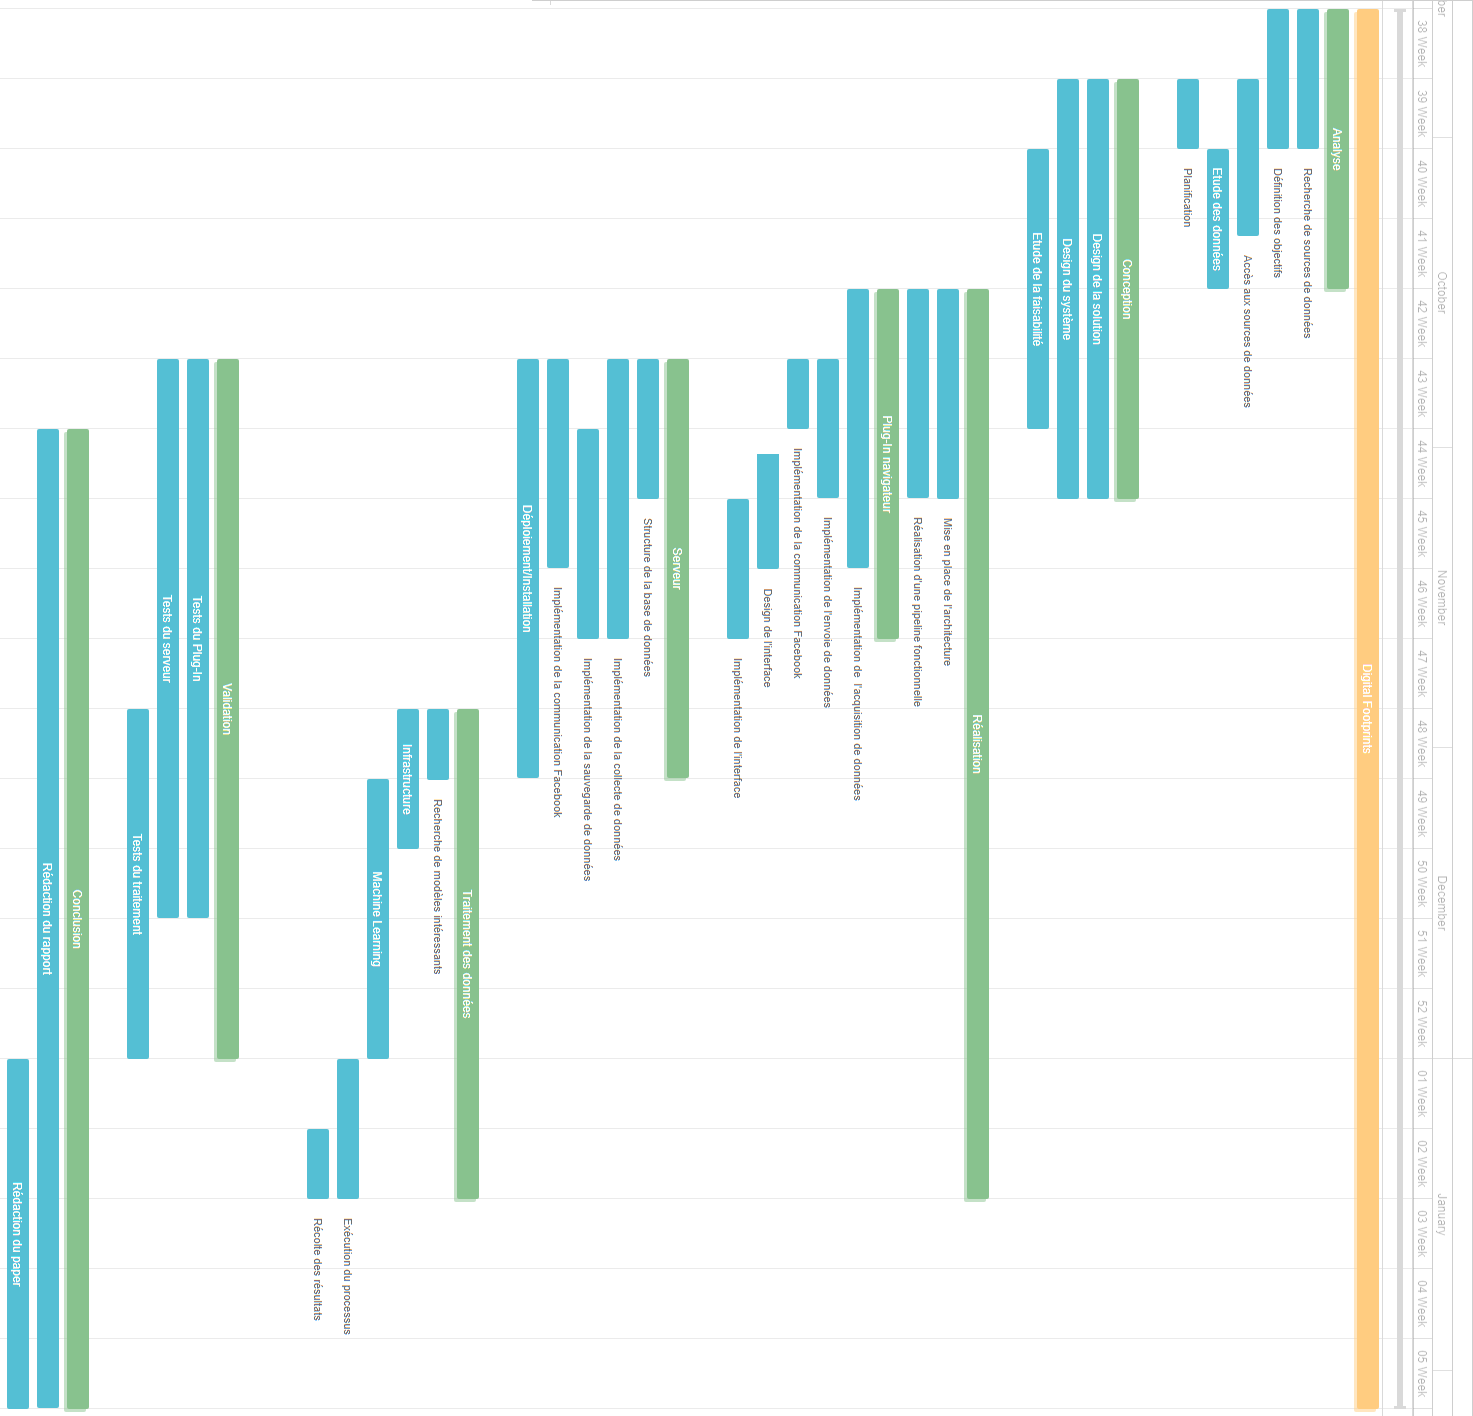
\includegraphics[width=0.95\textwidth]{images/annexes/cdc/newGantt}